\documentclass[12pt, notitlepage]{article}
\usepackage{amsmath}
\usepackage{amssymb}
\usepackage{graphicx}
\usepackage{amsthm}
\usepackage{listings}
\usepackage{color}
\usepackage{float}
\usepackage{caption}
\usepackage{subcaption}

\definecolor{dkgreen}{rgb}{0,0.6,0}
\definecolor{gray}{rgb}{0.5,0.5,0.5}
\definecolor{mauve}{rgb}{0.58,0,0.82}

\lstset{
	frame=single,
	language=Java,
	belowskip=3mm,
	showstringspaces=false,
	columns=flexible,
	captionpos=b,
	basicstyle={\small\ttfamily},
	numbers=left,
	numbersep=5pt,
	%numbers=none,
	numberstyle=\tiny\color{gray},
	keywordstyle=\color{blue},
	commentstyle=\color{dkgreen},
	stringstyle=\color{mauve},
	breaklines=true,
	breakatwhitespace=true,
	tabsize=3
}


\providecommand{\abs}[1]{\lvert#1\rvert}
\providecommand{\norm}[1]{\lVert#1\rVert}

\newtheorem{thm}{Theorem}
\newtheorem{lemma}[thm]{Lemma}
\newtheorem{fact}[thm]{Fact}
\newtheorem{cor}[thm]{Corollary}
\newtheorem{eg}{Example}
\newtheorem{ex}{Exercise}
\newtheorem{defi}{Definition}
\newtheorem{hw}{Homework}
\newenvironment{sol}
  {\par\vspace{3mm}\noindent{\it Solution}.}{\qed}

\newcommand{\fib}{\mbox{fib}}
\newcommand{\ov}{\overline}
\newcommand{\cb}{{\cal B}}
\newcommand{\cc}{{\cal C}}
\newcommand{\cd}{{\cal D}}
\newcommand{\ce}{{\cal E}}
\newcommand{\cf}{{\cal F}}
\newcommand{\ch}{{\cal H}}
\newcommand{\cl}{{\cal L}}
\newcommand{\cm}{{\cal M}}
\newcommand{\cp}{{\cal P}}
\newcommand{\cz}{{\cal Z}}
\newcommand{\eps}{\varepsilon}
\newcommand{\ra}{\rightarrow}
\newcommand{\la}{\leftarrow}
\newcommand{\Ra}{\Rightarrow}
\newcommand{\dist}{\mbox{\rm dist}}
\newcommand{\bn}{{\mathbf N}}
\newcommand{\bz}{{\mathbf Z}}

\setlength{\parindent}{0pt}
%\setlength{\parskip}{2ex}
\newenvironment{proofof}[1]{\bigskip\noindent{\itshape #1. }}{\hfill$\Box$\medskip}

\usepackage{enumerate,fullpage, proof}
\newcommand{\Infer}[2]{\infer{#2}{#1}}

\title{Homework 4}
\author{Team: nogg\footnote{E-mail: \texttt{kimi.ysma@gmail.com}}\footnote{Team member: Ma Yesheng, Zhao Ming, Hu Hu, Zou Yikai, Fan Minghua}}

\begin{document}

{\bf\small CS214: Algorithms and Complexity}\hfill{\bf\small 2016 Fall}
{\let\newpage\relax\maketitle}

\textbf{Exercise 1}
\begin{sol}
	
\qquad If there are intersections of s-r-flow and r-t-flow, then there must be circles which contains $r$. Remove these circles and it won't change the flow value form $s$ to $t$. Thus, this lemma is proved.

\end{sol}\\

\textbf{Exercise 2}
\begin{sol}\\
At first, we need to prove \textbf{Hall's Theorem}.\\
\textbf{Hall's Theorem}: A bipartite graph $G$ with vertex sets $V_1$ and $V_2$ contains a complete matching
from $V_1$ to $V_2$ if and only if it satisfies Hall's condition\\
\centerline{$|\Gamma (S)| >= |S|\ for\ every\ S \subset V$}
\begin{proof}
First, we observe that Hall’s condition is clearly necessary. To prove that it is also sufficient, we use induction on $m$. The theorem is true for $m = 1$, so assume that $G$ satisfies Hall’s condition and that $m = |V1| >= 2$.

\qquad \textbf{Case 1.}Suppose that for all proper subsets $S _6 \neq \O$ of $V_1$,\\
\centerline{$|\Gamma(S)| >= |S| + 1$}
Then we can start with an arbitrary edge $e = v_1v_2 \in E$, and put $e$ in $M$. The graph $G_0 = G- \{v_1, v_2\}$ satisfies Hall ’s condition, so we can complete the matching by induction.

\qquad \textbf{Case 2.}Suppose that for some proper subset $T \neq \O$ of $V_1$,\\
\centerline{$|\Gamma (T)| = |T|$}
Applying the induction hypothesis to $G' = G[T \cup \Gamma (T)]$ and $G'' = G[(V1 \backslash T) \cup (V2 \backslash \Gamma (T))]$, we obtain two disjoint matchings containing $|T|$ and $m-|T|$ edges respectively, whose union is a complete matching from $V_1$ to $V_2$.
\end{proof}

Then, we'll prove this exercise.\\
Assume that $|V_1| <= |V_2|$. Because $|V_1|*d_1 = |V_2|*d_2$, so $d_1 >= d_2$.\\
For any vertex subset $V_1'$ that $V_1'\subset V_1$, the neighbor set of $V_1'$ is $\Gamma (V_1')$. Then there must be
\centerline{$|V_1'|*d_1 = \sum\limits^{|\Gamma (V_1')|}_{i=1}d_i$}
where $d_i$ is the number of edges that connect to the vertice in $V_1'$.\\
Because of $d_i <= d_2$, then\\
\centerline{$|V_1'|*d_1 = \sum\limits^{|\Gamma (V_1')|}_{i=1}d_i <= |\Gamma (V_1')| * d_2$}
Also because of $d_1 >= d_2$ that mentioned above, then $|V_1'| <= |\Gamma (V_1')|$.\\
According to \textbf{Hall's Theorem},  $G$ contains a matching of size $min(|V_1|, |V_2|)$.

\end{sol}


\textbf{Exercise 3}
\begin{sol}\\
First, since there is no edge between nodes at the same level, so we can simply regard set $L_i$ and set $L_{i+1}$ as two parts. Then we need to prove that this bipartite graph contains a matching of size $|L_i|=\binom{n}{i}$.\\
\textbf{OBSERVATION:}\\
1. $|L_i|\leq |L_{i+1}|$.\\
2. $\forall v\in L_i$, $|\{u|(v,u)\in E, u\in L_{i+1}\}|=\binom{n-i}{1}$.\\
3. $\forall v\in L_{i+1}$, $|\{u|(v,u)\in E, u\in L_i\}|=\binom{i+1}{1}$.\\
Then according to Exercise 2, we know that this bipartite graph contains a matching of size $min(|L_i|,|L_{i+1}|)=|L_i|=\binom{n}{i}$.
\end{sol}\\


\textbf{Exercise 4}
\begin{sol}
	\begin{enumerate}[1.]
		\item Since in this problem, all existing edges will not give any constraint to flow, we can give a infinite capacity for all existing edges. We only need to take care of vertices since for all vertex $u$ there is a vertex capacity $c(u)$ which limits outflow from this vertex.\\
			To express this constraint with edge capacity, we replace every vertex $v$ with two vertices $v_{in}$ and $v_{out}$, where edge capacity $c_{in\rightarrow out} = c(v)$. Also we need to replace all edge $(u, v)$ with $u_{out}\rightarrow v_{in}$.\\
			Finally we solve the max flow with edge capacities in this new graph and get the new $s-t$ flow.
	\item Picture shown as follows:
		\begin{figure}
			\centering
			\begin{subfigure}{.5\textwidth}
				\centering
				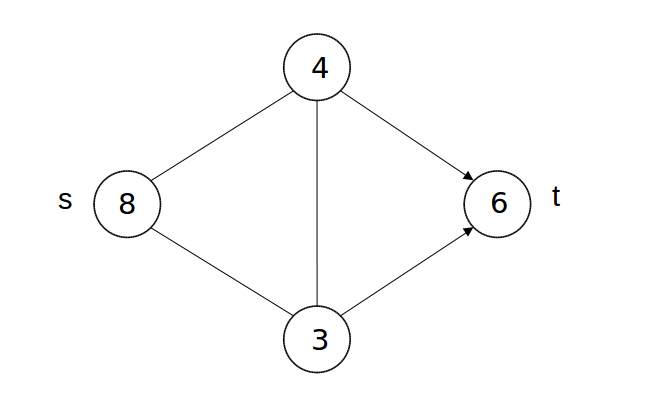
\includegraphics[width=0.8\linewidth]{dis1.png}
				\caption{vertex capacity graph}
			\end{subfigure}%
			\begin{subfigure}{.5\textwidth}
				\centering
				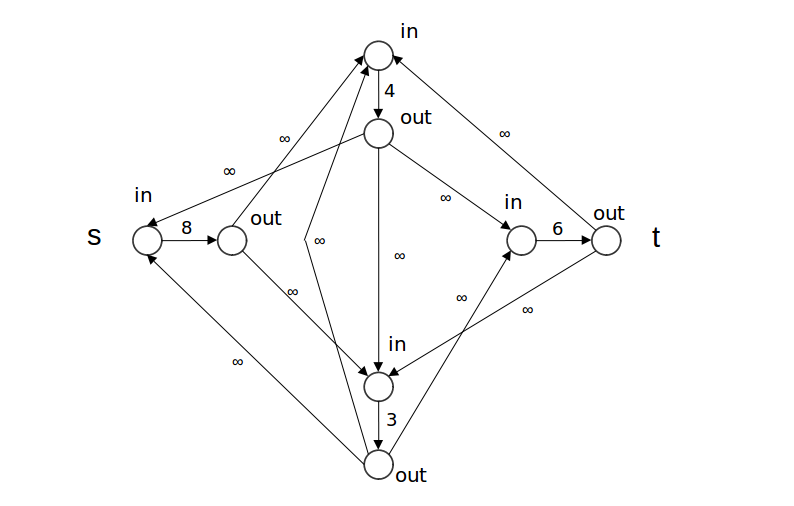
\includegraphics[width=1\linewidth]{dis2.png}
				\caption{converted edge capacity graph}
			\end{subfigure}
		\end{figure}
	\item Similar to previously introduced technique, we can construct a new graph to solve this problem:
		\begin{enumerate}[(1)]
			\item Replace each vertex $v$ with $v_{in}$ and $v_{out}$ and set edge capacity of it to be 1
			\item Replace each edge $(u, v)$ in the original graph to $u_{out}\rightarrow v_{in}$ with capacity $1$ in the new graph
			\item Sepecially, the source and destination of this graph are $v_{out}$ and $s$ respectively, where $s$ and $t$ are specified in the original graph
			\item Solve the max flow for the new graph from $s_{out}$ to $t$
		\end{enumerate}
		Since the graph construction and max flow can be solved in polynomial time, this solution for vertex disjoint paths can be solved in polynomial time.
	\end{enumerate}
\end{sol}


\textbf{Exercise 5}
\begin{sol}
	We prove this by considering a matching between $L_i$ and $L_{i+1}$. Since $\binom{n}{i}$ is the maximum number of vertices in $L_i$, we only need to prove that there exist such paths.\\
	For each vertex $v$ in $L_{j}$ where $(i\leq j\leq n-i)$, considering the property of Hamming code, $v$'s neighbor in the next level $L_{j+1}$ should be $\binom{n-j}{1}$.\\
	Since we only care about those $\binom{n}{i}$ paths from $L_i$ which is the maximal possible number of disjoint paths, 
	we can then consider the matching where $L$ and $R$ are vertex set of size $\binom{n}{i}$ rather than consider all the vertices in $L_j$ and $L_{j+1}$. 
	Then for all vertices that belongs to one of the vertex disjoint paths, we can conclude that there exist a matching from these vertices to vertices in $L{i+1}$ from Hall's theorem.\\
	Thus for each level there is such a matching of size $\binom{n}{i}$. Therefor there are $\binom{n}{i}$ such paths.

\end{sol}

\textbf{Exercise 6}
\begin{sol}
    \\1.Reduce it to a max flow problem.\\
    \textbf{Observation.} We have noticed that for a orientation graph, there must be at least a directed edge for each undirected edge. Every directed edge will increase the indegree of a node.\\\\
    So we came up the following solution:\\
    Firstly, we number the nodes with 1,2,3...\\
    Secondly, we number the edges with a,b,c,...\\
    Thirdly, we draw the picture with two sets, one set is the set of numbers, one set is the set of characters.\\
    Fourthly, we connect the two sets with directed edge for those joint in the undirected graph. For example, we have a edge named c and its two nodes are 5 and 7, then we add the directed edge from c to 5 and c to 7. All the directed edges are from characters to numbers. And every edge's capacity is 1.\\
    Fifthly, we add a start node s and the directed edges from s to all the character nodes. These edges' capacity is 2. And we add an end node t and the directed edges from number nodes to t.\\
    Finally, using the max-flow algorithm to find a max flow of this network, and specially while choosing the next path, we prior choose the path containing the character node which have not been added the the flow.\\
    And we check the flow to find all the character-number directed flow, and check whether all the character nodes have been included. If not, then there is no feasible orientation, then draw the feasible orientation with the directed edge which is included in the max flow.\\
    We choose the graph in the problem as an example.\\
    \begin{figure}[H]
	\center
	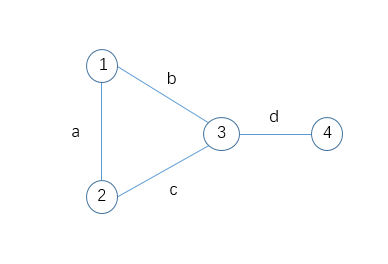
\includegraphics[width=0.6\linewidth]{6-1.png}\vspace{-10pt}
	\caption{} \nonumber\label{fig:first graph}\vspace{-10pt}
    \end{figure}
    \begin{figure}[H]
	\center
	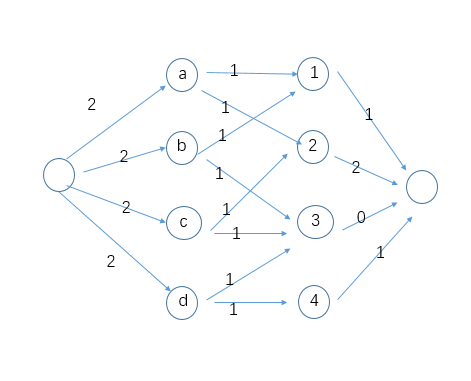
\includegraphics[width=0.6\linewidth]{6-2.png}\vspace{-10pt}
	\caption{} \nonumber\label{fig:second graph}\vspace{-10pt}
    \end{figure}
    And we can get the max flow including b-1, a-2, c-2, d-4.\\So we get the feasible orientation just like in the problem.\\
    Because finding the max flow has a polynomial-time algorithm, so the whole algorithm is polynomial-time.\\
    \\2.Reduce it to a maximum matching.\\
    We can just number the edges and nodes just like above, but there are some differences in constructing the directed graph.\\
    The first set are just character nodes set, and for the second number set, we just duplicate the node by its indegree size times, for example, if its max indegree is 5, then we get 5 same node in the second set. \\
    As for adding the edges, just like above.\\
    Then find the max matching of these graph. If the matching covers all the character node (which is edge), then there is a feasible orientation graph, otherwise there is not such a graph.\\
    We can still choose the graph in the problem as an example.\\
    Here is the constructing result.\\
    \begin{figure}[H]
	\center
	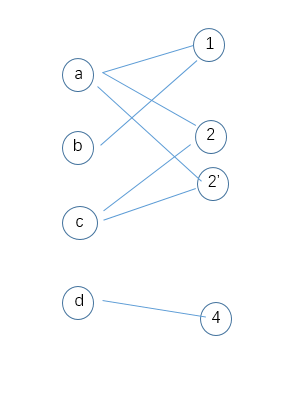
\includegraphics[width=0.6\linewidth]{6-3.png}\vspace{-10pt}
	\caption{} \nonumber\label{fig:third graph}\vspace{-10pt}
    \end{figure}
    And we can get the max matching $d-4, b-1, a-2, c-2'$.\\
    According to the max matching, we can get the feasible orientation graph and vice verse.\\
    Because finding the max matching has a polynomial-time algorithm, so the whole algorithm is polynomial-time.\\
\end{sol}


\textbf{Exercise 7}
\begin{sol}
\begin{enumerate}[1.]
\item
Graph is given below:
\begin{figure}[H]\centering
	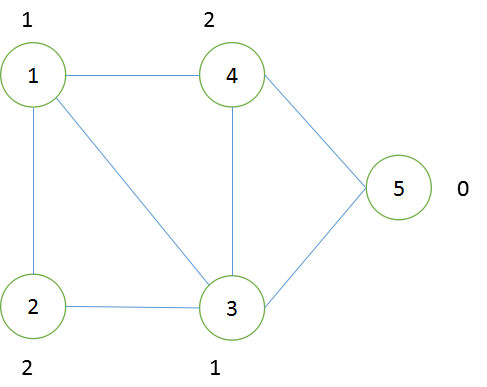
\includegraphics[width=7cm]{1.png}
	\caption{graph with degree constraints which has no feasible orientation}
\end{figure}
\item
\textbf{STATEMENT:} G has no feasible orientation with respect to c if and only if some set $X\subseteq E$ satisfis: $|X|>\sum_{v\in V(X)}c(v)$
\item
\textbf{PROOF:} \\
According to Exercise 6, by constructing a flow network, in which every edge's capacity is 1 and every vertex has as many copies as its degree constraint, or constructing a bipartite graph, we can reduce the problem about finding a feasible orientation to a problem about finding a max flow or a maximum matching which contains all the edges.\\
Like this:
\begin{figure}[H]\centering
	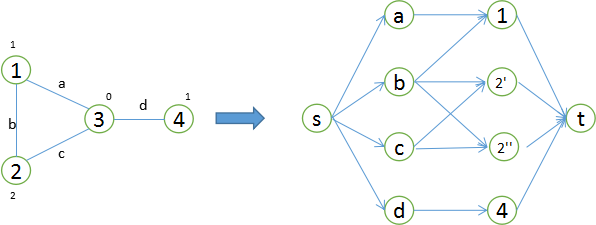
\includegraphics[width=12cm]{2.png}
	\caption{Using exercise 6's example to construct a flow network}
\end{figure}
\begin{figure}[H]\centering
	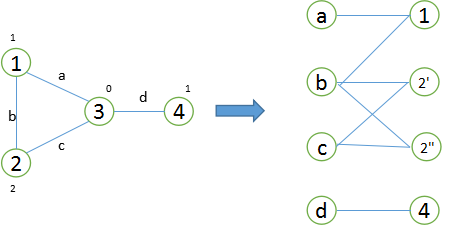
\includegraphics[width=12cm]{3.png}
	\caption{Using exercise 6's example to construct a bipartite graph}
\end{figure}
Then use Hall's Therrem. In bipartite graph $G'(E,V')$($V'$ is the vertex set containing all the copies of vertex in origin graph G), if there is no matching of size $|E|$, then some set $X\subseteq E$ has $|X|>|\Gamma(X)|$. It's obvious that in this bipartite graph, $\Gamma(X)$ contains all the vertices(and their copies) which is contained in some edge in set X. In other word, we get $|X|>\sum_{v\in V(X)}c(v)$. Vice Versa.
\end{enumerate}
\end{sol}\\

\textbf{Exercise 8}
\begin{sol}\\
We can reduce this problem to a maximum matching problem which is similar to ex6 and ex7.\\
Firstly, construct the graph as following steps.
\begin{enumerate}[1.]
 	\item Calculate the remained matches that team 1 needs to finish, $m_r = \sum_{i=2}^{n}m_{1,i}$.
 	\item Use a vertex to represent a team except team 1. $v_2,v_3,...,v_n$.
 	\item Give each vertex the in-degree constraint $c$, where $c_i = m_r + score_1 - score_i$. (Here $c_i$ represents the matches that team $i$ can win in the future in but score should not be more than team 1.)
 	\item Use indirect edges to connect these vertice. The number of edges between $v_i$ and $v_j$ is $m_{i,j}$.
\end{enumerate}

Then, the problem is reduced to find a feasible orientation of this graph. That is to say, if we can find a feasible orientation of this graph, then team 1 is possible to be the unique winner. On the contrary, it is impossible.\\
According to ex6, feasible orientation problem can be reduced to a maximum matching problem, which can be solved in polynomial time.



\end{sol}\\

\end{document}

